% Options for packages loaded elsewhere
\PassOptionsToPackage{unicode}{hyperref}
\PassOptionsToPackage{hyphens}{url}
%
\documentclass[
]{article}
\usepackage{lmodern}
\usepackage{amssymb,amsmath}
\usepackage{ifxetex,ifluatex}
\ifnum 0\ifxetex 1\fi\ifluatex 1\fi=0 % if pdftex
  \usepackage[T1]{fontenc}
  \usepackage[utf8]{inputenc}
  \usepackage{textcomp} % provide euro and other symbols
\else % if luatex or xetex
  \usepackage{unicode-math}
  \defaultfontfeatures{Scale=MatchLowercase}
  \defaultfontfeatures[\rmfamily]{Ligatures=TeX,Scale=1}
\fi
% Use upquote if available, for straight quotes in verbatim environments
\IfFileExists{upquote.sty}{\usepackage{upquote}}{}
\IfFileExists{microtype.sty}{% use microtype if available
  \usepackage[]{microtype}
  \UseMicrotypeSet[protrusion]{basicmath} % disable protrusion for tt fonts
}{}
\makeatletter
\@ifundefined{KOMAClassName}{% if non-KOMA class
  \IfFileExists{parskip.sty}{%
    \usepackage{parskip}
  }{% else
    \setlength{\parindent}{0pt}
    \setlength{\parskip}{6pt plus 2pt minus 1pt}}
}{% if KOMA class
  \KOMAoptions{parskip=half}}
\makeatother
\usepackage{xcolor}
\IfFileExists{xurl.sty}{\usepackage{xurl}}{} % add URL line breaks if available
\IfFileExists{bookmark.sty}{\usepackage{bookmark}}{\usepackage{hyperref}}
\hypersetup{
  pdftitle={Homework 1},
  pdfauthor={Jeremy Lin},
  hidelinks,
  pdfcreator={LaTeX via pandoc}}
\urlstyle{same} % disable monospaced font for URLs
\usepackage[margin=1in]{geometry}
\usepackage{longtable,booktabs}
% Correct order of tables after \paragraph or \subparagraph
\usepackage{etoolbox}
\makeatletter
\patchcmd\longtable{\par}{\if@noskipsec\mbox{}\fi\par}{}{}
\makeatother
% Allow footnotes in longtable head/foot
\IfFileExists{footnotehyper.sty}{\usepackage{footnotehyper}}{\usepackage{footnote}}
\makesavenoteenv{longtable}
\usepackage{graphicx,grffile}
\makeatletter
\def\maxwidth{\ifdim\Gin@nat@width>\linewidth\linewidth\else\Gin@nat@width\fi}
\def\maxheight{\ifdim\Gin@nat@height>\textheight\textheight\else\Gin@nat@height\fi}
\makeatother
% Scale images if necessary, so that they will not overflow the page
% margins by default, and it is still possible to overwrite the defaults
% using explicit options in \includegraphics[width, height, ...]{}
\setkeys{Gin}{width=\maxwidth,height=\maxheight,keepaspectratio}
% Set default figure placement to htbp
\makeatletter
\def\fps@figure{htbp}
\makeatother
\setlength{\emergencystretch}{3em} % prevent overfull lines
\providecommand{\tightlist}{%
  \setlength{\itemsep}{0pt}\setlength{\parskip}{0pt}}
\setcounter{secnumdepth}{-\maxdimen} % remove section numbering
\usepackage{booktabs}
\usepackage{longtable}
\usepackage{array}
\usepackage{multirow}
\usepackage{wrapfig}
\usepackage{float}
\usepackage{subfig}
\floatplacement{figure}{H}
\usepackage{subfig}
\usepackage{booktabs}
\usepackage{longtable}
\usepackage{array}
\usepackage{multirow}
\usepackage{wrapfig}
\usepackage{float}
\usepackage{colortbl}
\usepackage{pdflscape}
\usepackage{tabu}
\usepackage{threeparttable}
\usepackage{threeparttablex}
\usepackage[normalem]{ulem}
\usepackage{makecell}
\usepackage{xcolor}

\title{Homework 1}
\author{Jeremy Lin}
\date{1/15/2021}

\begin{document}
\maketitle

\hypertarget{problem-1}{%
\subsection{Problem 1}\label{problem-1}}

\hypertarget{compute-the-posterior-distribution-pthetax3.}{%
\subsubsection{\texorpdfstring{Compute the posterior distribution
\(p(\theta|x=3)\).}{Compute the posterior distribution p(\textbackslash theta\textbar x=3).}}\label{compute-the-posterior-distribution-pthetax3.}}

\begin{longtable}[]{@{}llllll@{}}
\toprule
\(\theta\) & 0.3 & 0.4 & .5 & .6 & .7\tabularnewline
\midrule
\endhead
\(p(\theta)\) & 0.022 & 0.038 & 0.831 & 0.057 & 0.051\tabularnewline
\bottomrule
\end{longtable}

\hypertarget{compute-the-posterior-mean-ethetax3-which-can-be-assumed-as-a-possible-estimator-of-the-population-proportion-based-on-the-observed-data.}{%
\subsubsection{\texorpdfstring{Compute the posterior mean,
\(E(\theta|x=3)\), which can be assumed as a possible estimator of the
population proportion, based on the observed
data.}{Compute the posterior mean, E(\textbackslash theta\textbar x=3), which can be assumed as a possible estimator of the population proportion, based on the observed data.}}\label{compute-the-posterior-mean-ethetax3-which-can-be-assumed-as-a-possible-estimator-of-the-population-proportion-based-on-the-observed-data.}}

\begin{align}
  E(\theta|x = 3) &= \sum \theta * p(\theta|x = 3) \\
  E(\theta|x = 3) &= 0.507778
\end{align}

\hypertarget{suppose-i-conduct-a-more-thorough-study-and-obtain-data-from-10-more-individuals.-among-them-eight-clicked-on-the-post.-based-on-the-currently-available-information-how-would-you-update-your-inference-on-the-parameter-theta}{%
\subsubsection{\texorpdfstring{Suppose I conduct a more thorough study,
and obtain data from 10 more individuals. Among them, eight clicked on
the post. Based on the currently available information, how would you
update your inference on the parameter
\(\theta\)?}{Suppose I conduct a more thorough study, and obtain data from 10 more individuals. Among them, eight clicked on the post. Based on the currently available information, how would you update your inference on the parameter \textbackslash theta?}}\label{suppose-i-conduct-a-more-thorough-study-and-obtain-data-from-10-more-individuals.-among-them-eight-clicked-on-the-post.-based-on-the-currently-available-information-how-would-you-update-your-inference-on-the-parameter-theta}}

The updated posterior distribution \(p(\theta|x = 8)\)

\begin{longtable}[]{@{}llllll@{}}
\toprule
\(\theta\) & 0.3 & 0.4 & .5 & .6 & .7\tabularnewline
\midrule
\endhead
\(p(\theta)\) & 0.001 & 0.007 & 0.653 & 0.124 & 0.214\tabularnewline
\bottomrule
\end{longtable}

\hypertarget{based-on-the-results-from-3-would-you-conclude-that-the-campaign-marketing-post-is-successful-or-youd-look-for-a-better-post-this-is-a-thought-provoking-question-at-this-point-try-your-best-about-to-answer-it}{%
\subsubsection{Based on the results from (3), would you conclude that
the campaign marketing post is successful, or you'd look for a better
post? {[}This is a thought-provoking question at this point; try your
best about to answer
it{]}}\label{based-on-the-results-from-3-would-you-conclude-that-the-campaign-marketing-post-is-successful-or-youd-look-for-a-better-post-this-is-a-thought-provoking-question-at-this-point-try-your-best-about-to-answer-it}}

To conclude that campaign marketing post is successful, I will use a cut
off of 50\% chance or greater that a person will click on the post
(\(\theta >0.6\). The probability of theres is more than 60\% chance a
person will click on the post is equal to 0.463, Therefore I think this
marketing is succesfull.

\hypertarget{problem-2}{%
\subsection{Problem 2}\label{problem-2}}

\hypertarget{based-on-the-interim-analysis-what-is-the-posterior-distribution-of-theta}{%
\subsubsection{\texorpdfstring{Based on the interim analysis, what is
the posterior distribution of
\(\theta\)?}{Based on the interim analysis, what is the posterior distribution of \textbackslash theta?}}\label{based-on-the-interim-analysis-what-is-the-posterior-distribution-of-theta}}

From interim analysis 20(y = 20) out of 30(n = 30) patients had a
positive outcome. Assume uniform prior on \(\theta\).

Posterior distribution : \[\theta|y \sim Beta(21, 11)\]

\hypertarget{what-is-a-possible-point-estimate-for-theta}{%
\subsubsection{\texorpdfstring{What is a possible point estimate for
\(\theta\)?}{What is a possible point estimate for \textbackslash theta?}}\label{what-is-a-possible-point-estimate-for-theta}}

Possible point estimate : \begin{align}
  E(\theta|y) = \frac{a+y}{a+b+n} 
  = \frac{21}{32}
  \approx 0.656
\end{align}

\hypertarget{find-the-5-and-95-quantiles-of-the-posterior-distribution.}{%
\subsubsection{Find the 5\% and 95\% quantiles of the posterior
distribution.}\label{find-the-5-and-95-quantiles-of-the-posterior-distribution.}}

The 5\% quantile is 0.5145839 and the 95\% quantile is 0.7866395

\hypertarget{in-the-continuation-of-the-trial-50-out-of-the-remaining-patients-have-had-a-positive-outcome.-what-is-the-updated-posterior-of-theta-what-is-a-possible-estimate-for-theta-find-the-5-and-95-quantiles-of-the-distribution.}{%
\subsubsection{\texorpdfstring{In the continuation of the trial, 50 out
of the remaining patients have had a positive outcome. What is the
updated posterior of \(\theta\)? What is a possible estimate for
\(\theta\)? Find the 5\% and 95\% quantiles of the
distribution.}{In the continuation of the trial, 50 out of the remaining patients have had a positive outcome. What is the updated posterior of \textbackslash theta? What is a possible estimate for \textbackslash theta? Find the 5\% and 95\% quantiles of the distribution.}}\label{in-the-continuation-of-the-trial-50-out-of-the-remaining-patients-have-had-a-positive-outcome.-what-is-the-updated-posterior-of-theta-what-is-a-possible-estimate-for-theta-find-the-5-and-95-quantiles-of-the-distribution.}}

The updated posterior \(\theta\) is : \[\theta|y \sim Beta(71, 31)\]
Possible point estimate : \begin{align}
  E(\theta|y) = \frac{a+y}{a+b+n} 
  = \frac{71}{102}
  \approx 0.696
\end{align}

The 5\% quantile is 0.619 and the 95\% quantile is 0.768

\hypertarget{based-on-the-results-from-the-analysis-does-the-treatment-appear-promising}{%
\subsubsection{Based on the results from the analysis, does the
treatment appear
promising?}\label{based-on-the-results-from-the-analysis-does-the-treatment-appear-promising}}

Since we are 90\% sure that the percentage of patient having a positive
outcome because of the treatment is between between 61.935\% and
76.841\%. therefore I believe that the treatment appear promising.

\hypertarget{problem-3}{%
\subsection{Problem 3}\label{problem-3}}

\hypertarget{describe-your-model-for-studying-the-clutch-success-probability-of-each-subject-including-the-likelihood-and-prior.}{%
\subsubsection{Describe your model for studying the clutch success
probability of each subject, including the likelihood and
prior.}\label{describe-your-model-for-studying-the-clutch-success-probability-of-each-subject-including-the-likelihood-and-prior.}}

We want to study the clutch success probability, i.e the proportion of
number of clutch success over the number of clutch attempts. For this
type of data, we assume Binomial likelihood, with a uniform prior
(Beta(1,1)) distribution. Therefore our likelihood function is :
\[L(y|\theta) \propto \theta^y (1-\theta)^{n-y} \] with prior
distribution \[\theta_{prior} \sim Beta(1,1)\]

\hypertarget{plot-the-posterior-distribution-of-the-clutch-success-probabilities-for-james-harden-and-le-bron-james.}{%
\subsubsection{Plot the posterior distribution of the clutch success
probabilities for James Harden and Le Bron
James.}\label{plot-the-posterior-distribution-of-the-clutch-success-probabilities-for-james-harden-and-le-bron-james.}}

\hypertarget{posterior-distribution-of-james-harden}{%
\paragraph{Posterior Distribution of James Harden
:}\label{posterior-distribution-of-james-harden}}

\[p(\theta|y) \sim Beta(73, 24) \] with the distribution plot:

\begin{flushleft}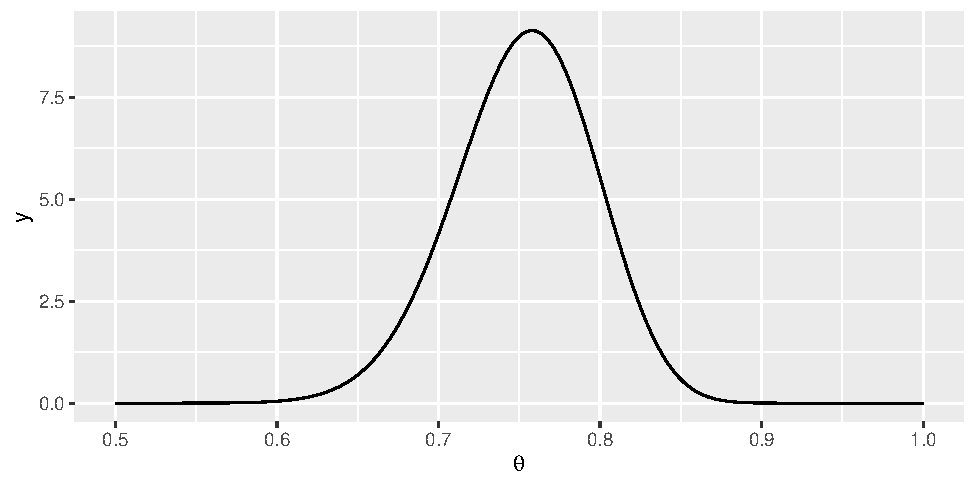
\includegraphics{homework_1_files/figure-latex/unnamed-chunk-2-1} \end{flushleft}

\hypertarget{posterior-distribution-of-lebron-james}{%
\paragraph{Posterior Distribution of Lebron
James}\label{posterior-distribution-of-lebron-james}}

\[p(\theta|y) \sim Beta(28, 13) \]

with the distribution plot:

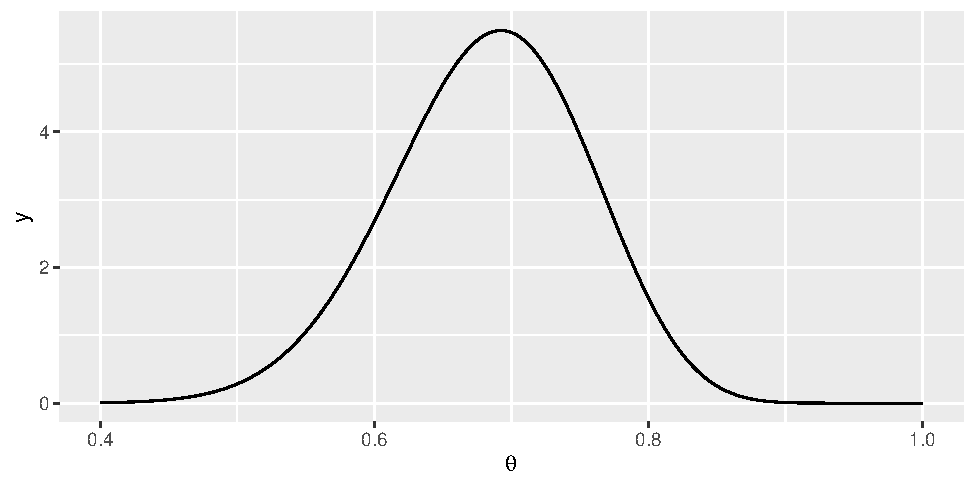
\includegraphics{homework_1_files/figure-latex/unnamed-chunk-4-1.pdf}

\hypertarget{summarize-the-posterior-distribution-for-each-player-in-a-table.-the-table-should-include-at-least-the-posterior-mean-and-the-5-25-50-75-95-posterior-quantiles.}{%
\subsubsection{\texorpdfstring{Summarize the posterior distribution
\emph{for each player} in a table. The table should include (at least)
the posterior mean and the (5\%, 25\%, 50\%, 75\%, 95\%) posterior
quantiles.}{Summarize the posterior distribution for each player in a table. The table should include (at least) the posterior mean and the (5\%, 25\%, 50\%, 75\%, 95\%) posterior quantiles.}}\label{summarize-the-posterior-distribution-for-each-player-in-a-table.-the-table-should-include-at-least-the-posterior-mean-and-the-5-25-50-75-95-posterior-quantiles.}}

Table 3 is the summary of the posterior distribution for each player.

\begin{table}[H]

\caption{\label{tab:unnamed-chunk-6}Player Summary}
\centering
\begin{tabular}[t]{lrrrrrr}
\toprule
Player & post\_mean & post\_5 & post\_25 & post\_50 & post\_75 & post\_95\\
\midrule
Russel Westbrook & 0.8441558 & 0.7718157 & 0.8180802 & 0.8471422 & 0.8734561 & 0.9062892\\
James Harden & 0.7525773 & 0.6779739 & 0.7240035 & 0.7543189 & 0.7830364 & 0.8212314\\
Kawhi Leonard & 0.8615385 & 0.7857443 & 0.8349456 & 0.8652532 & 0.8921340 & 0.9246310\\
LeBron James & 0.6829268 & 0.5597203 & 0.6354949 & 0.6859271 & 0.7335766 & 0.7958659\\
Isaiah Thomas & 0.8941176 & 0.8347164 & 0.8735612 & 0.8972081 & 0.9180112 & 0.9429563\\
\addlinespace
Stephen Curry & 0.8928571 & 0.7847000 & 0.8599061 & 0.9021872 & 0.9356802 & 0.9690216\\
Giannis Antetokoumpo & 0.6744186 & 0.5535649 & 0.6276477 & 0.6771455 & 0.7241164 & 0.7859418\\
John Wall & 0.7976190 & 0.7220548 & 0.7694267 & 0.7999885 & 0.8283730 & 0.8650869\\
Anthony Davis & 0.7321429 & 0.6310221 & 0.6937741 & 0.7349227 & 0.7735056 & 0.8237581\\
Kevin Durant & 0.7777778 & 0.6043586 & 0.7179257 & 0.7882150 & 0.8485597 & 0.9153549\\
\bottomrule
\end{tabular}
\end{table}

\hypertarget{do-you-find-evidence-that-any-of-the-players-have-a-different-clutch-percentage-than-overall-percentage-hint-test-the-hypothesis-that-the-probability-of-clutch-for-a-player-is-greater-than-their-corresponding-overall-proportion}{%
\subsubsection{\texorpdfstring{Do you find evidence that any of the
players have a different clutch percentage than overall percentage?
{[}\emph{Hint: test the hypothesis that the probability of ``clutch''
for a player is greater than their corresponding overall
proportion}{]}}{Do you find evidence that any of the players have a different clutch percentage than overall percentage? {[}Hint: test the hypothesis that the probability of ``clutch'' for a player is greater than their corresponding overall proportion{]}}}\label{do-you-find-evidence-that-any-of-the-players-have-a-different-clutch-percentage-than-overall-percentage-hint-test-the-hypothesis-that-the-probability-of-clutch-for-a-player-is-greater-than-their-corresponding-overall-proportion}}

Let the overall proportion be \(\pi\) , Table 4 is the probability of
clutch proportion is greater than their corresponding overall proportion
(\(p(\theta > \pi)\)). James Harden, Giannis Antetokoumpo, Anthony
Davis, and Kevin Durant has a pretty low probably that could indicate
that the player have a different clutch percentage than their
corresponding overall percentage. This could due because these players
tend to avoid taking clutch shots (low number of clutch attempt), with
an exception of James Harden Who have the most attempt through all the
player.

Table 4 also provided the 90\% credible interval of clutch percentage
and James Harden overall proportion is the only one inside the 90\% CI,
therefore we have a strong evidence that James Harden have a different
clutch percentage than his shot percentage.

\begin{table}[H]

\caption{\label{tab:unnamed-chunk-7}Player Summary}
\centering
\begin{tabular}[t]{lrrrr}
\toprule
Player & probability & post\_5 & post\_95 & overal\_proportion\\
\midrule
Russel Westbrook & 0.5207121 & 0.7718157 & 0.9062892 & 0.845\\
James Harden & 0.0090208 & 0.6779739 & 0.8212314 & 0.847\\
Kawhi Leonard & 0.3597559 & 0.7857443 & 0.9246310 & 0.880\\
LeBron James & 0.5645547 & 0.5597203 & 0.7958659 & 0.674\\
Isaiah Thomas & 0.3553753 & 0.8347164 & 0.9429563 & 0.909\\
\addlinespace
Stephen Curry & 0.5293229 & 0.7847000 & 0.9690216 & 0.898\\
Giannis Antetokoumpo & 0.0833433 & 0.5535649 & 0.7859418 & 0.770\\
John Wall & 0.4907634 & 0.7220548 & 0.8650869 & 0.801\\
Anthony Davis & 0.1133361 & 0.6310221 & 0.8237581 & 0.802\\
Kevin Durant & 0.1542541 & 0.6043586 & 0.9153549 & 0.875\\
\bottomrule
\end{tabular}
\end{table}

\end{document}
